
\documentclass[9pt]{beamer}
%\makeatletter
%\def\beamer@calltheme#1#2#3{%
%	\def\beamer@themelist{#2}
%	\@for\beamer@themename:=\beamer@themelist\do
%	{\usepackage[{#1}]{\beamer@themelocation/#3\beamer@themename}}}
%
%\def\usefolder#1{
%	\def\beamer@themelocation{#1}
%}
%\def\beamer@themelocation{}

%\usefolder{../config}

\usetheme[
block=fill,
titleformat=regular,
progressbar=frametitle
]{metropolis}
%\metroset[everytitleformat=regular] % regular, lowercase, uppercase ]
%\metroset[inner/block=fill]

%\setbeameroption{show notes} 
\usepackage{booktabs}
\usepackage[scale=2]{ccicons}

\usepackage{pgfplots}
\usepgfplotslibrary{dateplot}


%\ Hrvatski znakovi
\usepackage[utf8]{inputenc}
\usepackage[T1]{fontenc}
\usepackage[croatian]{babel}
\usepackage{todonotes}
\usepackage{amsmath}
\usepackage{amsfonts}
\selectlanguage{croatian} % american ngerman
\usepackage{todonotes}

% Koristenje Latin modern fonta
% Bez toga na nekim racunalima baca
% err: Font <taj i taj> at <mala velicina, npr4.0pt> not loadable: Metric (TFM) file not found. \end{frame}
\usepackage{lmodern}


\definecolor{RoyalBlue}{cmyk}{1, 0.50, 0, 0}
%\usepackage{natbib}
%\usepackage{bibentry}
\usepackage{scrextend}
\usepackage{hyperref}
%\usepackage[pdfa=true]{hyperref}
\hypersetup{%
    %draft, % = no hyperlinking at all (useful in b/w printouts)
    %colorlinks=true, 
    linktocpage=true, pdfstartpage=3, pdfstartview=FitV,%
    % uncomment the following line if you want to have black links (e.g., for printing)
    %colorlinks=false, linktocpage=false, pdfborder={0 0 0}, pdfstartpage=3, pdfstartview=FitV,% 
    breaklinks=true, pdfpagemode=UseNone, pageanchor=true, pdfpagemode=UseOutlines,%
    plainpages=false, bookmarksnumbered, bookmarksopen=true, bookmarksopenlevel=1,%
    hypertexnames=true, pdfhighlight=/O,%nesting=true,%frenchlinks,%
    %urlcolor=webbrown, linkcolor=RoyalBlue, citecolor=webgreen, %pagecolor=RoyalBlue,%
    %urlcolor=Blue, linkcolor=Blue, citecolor=Red, %pagecolor=Black,%
    %pdftitle={\myTitle},%
    %pdfauthor={\textcopyright\ \myName, \myUni, \myFaculty},%
    pdfsubject={},%
    pdfkeywords={},%
    pdfcreator={pdfLaTeX},%
    pdfproducer={LaTeX with hyperref and classicthesis}, %
    unicode = true 
} 

%\usepackage[pdftex]{graphicx}
% declare the path(s) where your graphic files are
\graphicspath{{./}{./figures/}}


\newcommand{\executeiffilenewer}[3]{%
	\ifnum\pdfstrcmp{\pdffilemoddate{#1}}%
	{\pdffilemoddate{#2}}>0%
	{\immediate\write18{#3}}\fi%
}
\newcommand{\includesvg}[1]{%
	\executeiffilenewer{#1.svg}{#1.pdf}%
	{inkscape -z -C --file=#1.svg %
		--export-pdf=#1.pdf --export-latex}%
	\input{#1.pdf_tex}%
}


% http://tex.stackexchange.com/questions/83882/how-to-highlight-python-syntax-in-latex-listings-lstinputlistings-command

\usepackage{listings}
\usepackage{color}
\usepackage[semibold]{sourcecodepro}

% Default fixed font does not support bold face
\DeclareFixedFont{\ttb}{T1}{txtt}{bx}{n}{12} % for bold
\DeclareFixedFont{\ttm}{T1}{txtt}{m}{n}{12}  % for normal
% Custom colors
\definecolor{deepblue}{rgb}{0,0,0.5}
\definecolor{deepred}{rgb}{0.6,0,0}
\definecolor{deepgreen}{rgb}{0,0.5,0}


% Python style for highlighting
\newcommand\pythonstyle{\lstset{
		language=Python,
		basicstyle=\small\ttfamily,
		otherkeywords={self},             % Add keywords here
		keywordstyle=\small\ttfamily\color{deepblue},
		emph={MyClass,__init__},          % Custom highlighting
		emphstyle=\small\ttfamily\color{deepred},    % Custom highlighting style
		stringstyle=\color{deepgreen},
		frame=tb,                         % Any extra options here
		showstringspaces=false            % 
	}}
	
	
	% Python environment
	\lstnewenvironment{python}[1][]
	{
		\pythonstyle
		\lstset{#1}
	}
	{}
	
	% Python for external files
	\newcommand\pythonexternal[2][]{{
			\pythonstyle
			\lstinputlisting[#1]{#2}}}
	
	% Python for inline
	\newcommand\pythoninline[1]{{\pythonstyle\lstinline!#1!}}
%\documentclass[ucs]{beamer}
%\usetheme[menuwidth={0.3\paperwidth}]{erlangen}
%\setbeamercovered{transparent=20} 

\usepackage{amsmath,amsfonts,amsthm,amssymb}
\usepackage{setspace}
\usepackage{Tabbing}
\usepackage{fancyhdr}
\usepackage{lastpage}
\usepackage{extramarks}
\usepackage{chngpage}
\usepackage{soul,color}
\usepackage{graphicx,float,wrapfig}
\usepackage{xcolor}
\usepackage[normalem]{ulem}
\usepackage{mathtools}

\definecolor{erlangenlyellow}{RGB}{123, 25, 121}
%\usepackage[utf8x]{inputenc}
%\usepackage{default}
%\usepackage[T1]{fontenc}

\usepackage{verbatim}
\usepackage{listings}


\usepackage{subcaption}
\usepackage{lmodern}

\title{Uklanjanje skrivenih linija i površina i još ponešto}

\subtitle{how Occam would be ashamed}
\institute{Računalna grafika}

% Delete this, if you do not want the table of contents to pop up at
% the beginning of each subsection:
%\AtBeginSubsection[]
%{
%  \begin{frame}<beamer>{Outline}
%    \tableofcontents[currentsection,currentsubsection]
%  \end{frame}
%}
%
%\AtBeginSection[]
%{
%  \begin{frame}<beamer>{Outline}
%    \tableofcontents[currentsection]
%  \end{frame}
%}

\begin{document}
\begin{frame}
 \titlepage
\end{frame}

\begin{frame}{Sadržaj}
  \tableofcontents
  % You might wish to add the option [pausesections]
\end{frame}
\section{Uvod}
\begin{frame}{Problem}
	\begin{center}
		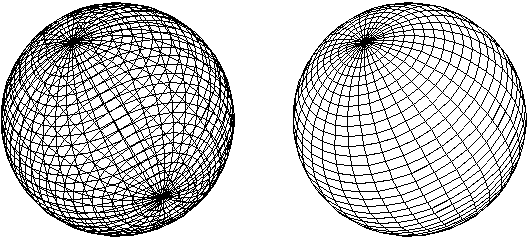
\includegraphics[height=4cm]{./slike/meshSpheres.png}
	\end{center}
\end{frame}

\begin{frame}{Motivacija}
	\begin{figure}
		\centering
		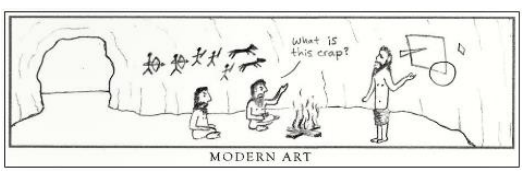
\includegraphics[width=0.9\linewidth]{./slike/modern_art}
%		\caption{}
%		\label{fig:modernart}
	\end{figure}
	
\end{frame}
\begin{frame}{Uklanjanje skrivenih linija i površina}
	\begin{block}{Osnove postupaka uklanjanja skrivenih linija i površina}
		\begin{itemize}
			\item geometrijska izračunavanja – uspostavljaju odnos između poligona, bridova i točaka (“containment test”)
			\item geometrijsko uređivanje (“geometric sorting”)
			\item postupci pretraživanja (“search algorithms”)
			\item međusoban ovisnost i obilježja (“coherence”)
		\end{itemize}
	\end{block}
\end{frame}

\begin{frame}{Uklanjanje contd.}
	\begin{block}{Određivanje vidljivosti}
		\begin{itemize}
			\item uklanjanje objekata izvan piramide pogleda (dijelova poligona)
			\item uklanjanje stražnjih pogona (eng. back face culling)
			\item brzi, jednostavni postupci za rješavanje trivijalnih slučajeva (npr. Min-maks provjera)
			\item promjena složenosti prikaza ovisno o udaljenosti (eng. LOD-level of detail)
		\end{itemize}
	\end{block}
	
	\begin{block}{Gruba podjela:}
		\begin{itemize}
			\item postupci u prostoru objekta 3D
			\item postupci u prostoru slike (projekcije) 2D
		\end{itemize}
	\end{block}
\end{frame}

\begin{frame}{Uklanjanje contd.}
	\begin{block}{Slični postupci:}
		\begin{itemize}
			\item odsijecanje (engl. clipping)
			\item  detekcije sudara tj. kolizije (engl. collision detection)
			\item bačene sjene
		\end{itemize}
	\end{block}
	\begin{block}{Geometrijska izračunavanja}
		Čine osnovu u postupcima uklanjanja skrivenih linija i poligona (u prostoru projekcije ili scene)
		\begin{itemize}
			\item položaj točke prema pravcu ili ravnini, prema poligonu ili tijelu
			\item položaj dužine prema pravcu ili ravnini, prema  poligonu ili tijelu
			\item Booleove operacije dvaju tijela (solid modelling)
			\item određivanje orijentacije poligona (u projekciji)
		\end{itemize}
	\end{block}
\end{frame}
\section{Poligon}
\begin{frame}{Poligon}
	Poligon se definira listom točaka $T_i$ koje su povezane bridovima $b_i$ na sljedeći način:
	\begin{align*}
	b_i \ldots \left\{ \begin{array}{cc}
	T_i, T_{i+i} & 0 < i < n \\
	Ti, T_0 & i = n
	\end{array}\right.
	\end{align*}
	Jednadžba pravca brida:
	\begin{align*}
	T_b= \left\{ \begin{array}{cc}
	(T_{i+i}-T_i)\lambda + T_i & 0 < i < n \\
	(T_0-T_i)\lambda + T_i & i = n
	\end{array}\right.
	\end{align*}
	Ovdje je $T_b$ proizvoljna točka pravca, ali samo za  $0 \leq \lambda \leq 1$, točka pripada bridu.
\end{frame}

\begin{frame}{Poligon}
	Pravac se dobije i kao vektorski produkt dvije točke:
	\begin{align*}
	T_i \times T_{i+1} & = \begin{bmatrix}
	 		\vec{i} & \vec{j}  & \vec{k}\\ 
	 		T_{i, 1} & T_{i, 2} & 1 \\
	 		T_{i+1, 1} & T_{i+1, 2} & 1 \end{bmatrix} \\
	 		 & = \begin{bmatrix}
	 		 \vec{i} & \vec{j}  & \vec{k}
	 		 \end{bmatrix} 
	 		 \begin{bmatrix}
	 		 T_{i, 2} - T_{i+1, 2}\\
	 		 -(T_{i, 1} - T_{i+1, 1})\\
	 		 T_{i,1}T_{i+1, 2}- T_{i,2}T_{i+1, 1} 
	 		 \end{bmatrix} \\
	 		 & = \begin{bmatrix}
	 		 \vec{i} & \vec{j}  & \vec{k}
	 		 \end{bmatrix}B_i \quad 0 < i < n
	\end{align*}
	\begin{align*}
	T_i \times T_0 & = \begin{bmatrix}
		\vec{i} & \vec{j}  & \vec{k}\\ 
		T_{i, 1} & T_{i, 2} & 1 \\
		T_{0, 1} & T_{0, 2} & 1 \end{bmatrix} \\
	& = \begin{bmatrix}
		\vec{i} & \vec{j}  & \vec{k}
	\end{bmatrix} 
	\begin{bmatrix}
		T_{i, 2} - T_{0, 2}\\
		-(T_{i, 1} - T_{0, 1})\\
		T_{i,1}T_{0, 2}- T_{i,2}T_{0, 1} 
	\end{bmatrix} \\
	& = \begin{bmatrix}
		\vec{i} & \vec{j}  & \vec{k}
	\end{bmatrix}B_i \quad i = n
\end{align*}
$B_i$ su koeficijenti pravca.
\end{frame}
\begin{frame}{Orijentacija vrhova poligona}
\begin{columns}
	\begin{column}[t]{0.5\textwidth}
		CW
	\begin{figure}
			\centering
			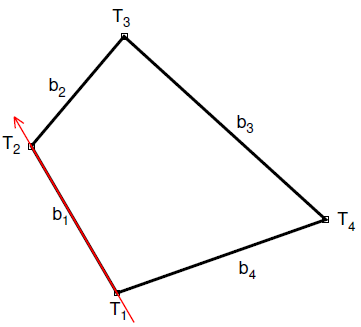
\includegraphics[width=0.8\textwidth]{slike/poligon_cw.png}
	\end{figure}
	\begin{align*}
		(\forall i) T_j \cdot B_i \leq 0 
	\end{align*}
	\end{column}
\begin{column}[t]{0.5\textwidth}
	CCW
	\begin{figure}
		\centering		
		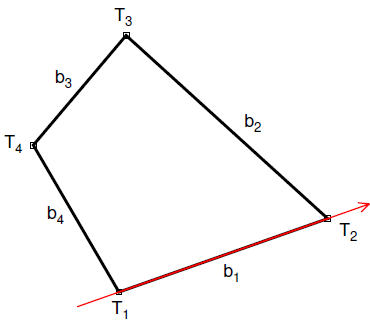
\includegraphics[width=0.8\textwidth]{slike/poligon_ccw.png}
	\end{figure}
	\begin{align*}
	(\forall i) T_j \cdot B_i \geq 0 
	\end{align*}
\end{column}
\end{columns}
gdje je 
\begin{align*}
j = \left\{ \begin{array}{cc}
j = i+2, & 0 < i < n-i \\
j = i-n +2, & n-1 \leq i \leq n 
\end{array}
\right.
\end{align*}
\end{frame}

\begin{frame}{Poligon konveksan?}
\begin{columns}
	\begin{column}[t]{0.5\textwidth}
		CW
		\begin{figure}
			\centering
			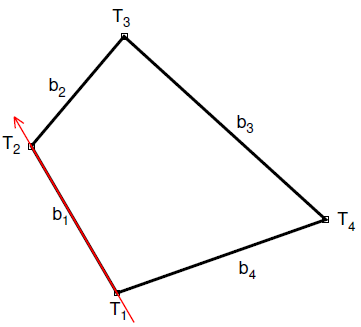
\includegraphics[width=0.8\textwidth]{slike/poligon_cw.png}
		\end{figure}
	Ako vrijedi 
	\begin{align*}
	(\exists i) T_j \cdot B_i < 0 ,
	\end{align*}
	Onda postoji barem jedan vrh takav da se nalazi ispod brida, odnosno, ako vrijedi za sve vrhove
		\begin{align*}
		(\forall i) T_j \cdot B_i \leq 0 
		\end{align*}
	\end{column}
	\begin{column}[t]{0.5\textwidth}
		CCW
		\begin{figure}
			\centering		
			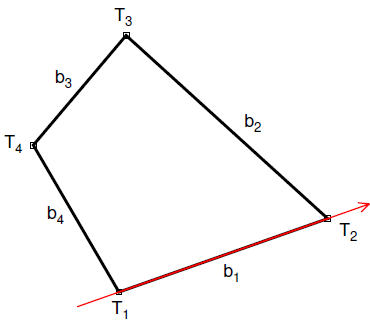
\includegraphics[width=0.8\textwidth]{slike/poligon_ccw.png}
		\end{figure}
		Ako vrijedi 
	\begin{align*}
	(\exists i) T_j \cdot B_i > 0 ,
	\end{align*}
	Onda postoji barem jedan vrh takav da se nalazi ispod brida, odnosno, ako vrijedi za sve vrhove
		\begin{align*}
		(\forall i) T_j \cdot B_i \geq 0 
		\end{align*}
	\end{column}
\end{columns}	
\end{frame}
\begin{frame}{Poligon konveksan?}
	\begin{block}{tldr;}
		Poligon je konveksan ako vrijedi:
		\begin{align*}
		(\forall i) T_j \cdot B_i \leq 0
		\end{align*}
		ili
		\begin{align*}
		(\forall i) T_j \cdot B_i \geq 0 
		\end{align*}
	\end{block}
	\begin{block}{još jedna sitnica}
		Ako smo sigurni da je poligon konveksan, onda orijentaciju vrhova možemo testirati tako da ispitamo samo jednu točku sa jednim bridom.
	\end{block}
\end{frame}
\begin{frame}{Provjera odnosa točke i poligona}
	\begin{block}{Korištenje sume kuteva}
		\begin{itemize}
			\item ako je $\sum_{i} \alpha_{i} = 0$, $P_{t}$ je izvan poligona
			\item ako je $\sum_{i} \alpha_{i} = 2\pi$, $P_{t}$ je unutar poligona 
		\end{itemize}
	\end{block}

\begin{block}{Koristimo skalarni produkt, samo za konveksne poligone}
	\begin{itemize}
		\item CW poligon: ako je $(\forall i) T_j \cdot B_i \geq 0$ točka je unutar poligona
	  \item CCW poligon: ako je $(\forall i) T_j \cdot B_i \leq 0$ točka je unutar poligona 
	\end{itemize}
\end{block}
\end{frame}

\section{Painter's algorithm}

\begin{frame}{Geometrijsko određivanje}
	
	\begin{center}
		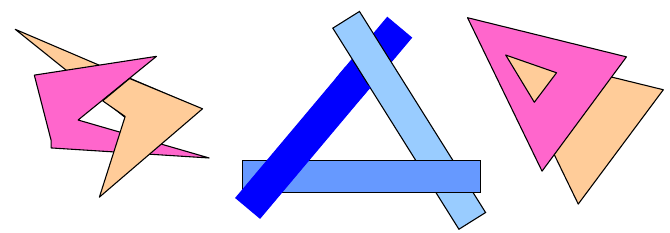
\includegraphics[height=3cm]{slike/03_geometrija_1.png}
	\end{center}
	Nakon iscrtavanja najudaljenijih poligona crtaju se redom sve bliži koji prekrivaju iscrtane poligone. 
	Primjer: Painter's algorithm
	Prednosti: prozirnost
	Nedostatak: suvišno iscrtavanje prekrivenih poligona, problem iscrtavanja površina ili probadanja
\end{frame}

\section{Provjera normale}
\begin{frame}{Provjera normale}
	\begin{block}{Cilj}
		Ne iscrtavati stražnje poligone nekog geometrijskog tijela.
	\end{block}
	\begin{block}{Pretpostavke}
		\begin{itemize}
			\item Tijelo je opisano nizom poligona
			\item Tijelo je konveksno
			\item Vrhovi poligona su zadani u CCW smjeru
		\end{itemize}
	\end{block}
	\begin{block}{Posljedica}
		\begin{itemize}
			\item Normale gledaju iz tijela prema van
			\item Normala koja je \textit{od očišta} pripada stražnjem poligonu
		\end{itemize}
	\end{block}
\end{frame}
\begin{frame}{Provjera normale}
	\begin{block}{Tehnikalije}
		\begin{itemize}
			\item Provjerava se kut koji zatvara normala poligona i vektor usmjeren iz središta poligona prema očištu
			\item poligon je stražnji ako $\vec{N}_P\cdot \cdot \vec{N} < 0$
			\item poligon je prednji ako $\vec{N}_P\cdot \cdot \vec{N} > 0$
			\item promatrač vidi poligon kao liniju $\vec{N}_P\cdot \cdot \vec{N} = 0$
		\end{itemize}
	\end{block}
	\begin{center}
		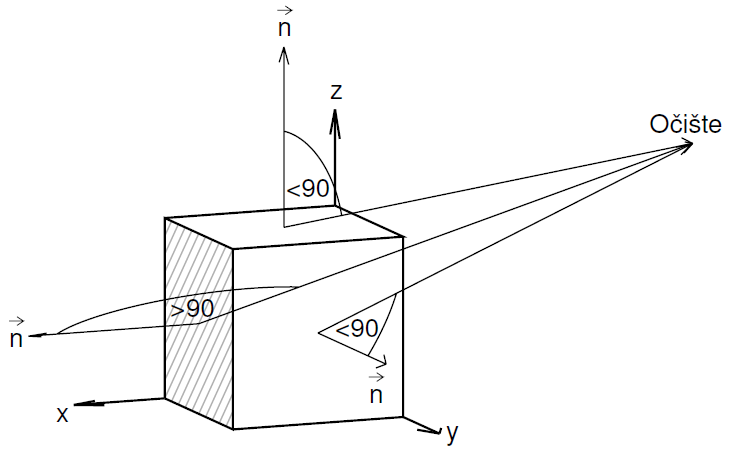
\includegraphics[height=3.5cm]{./slike/provjera_normala.png}
	\end{center}
\end{frame}

\begin{frame}{Provjera normale}
	\begin{block}{Drugi način}
		\begin{itemize}
			\item Kreiramo ravninu kojoj pripada poligon
			\item Uvrstimo položaj očišta u jednadžbu ravnine
			\item Ako je očište \textit{ispod}, poligon je stražnji
			\item Ako je očište \textit{iznad}, poligon je prednji
		\end{itemize}
	$\mathbf{T}\cdot \mathbf{R}$ - izrazi 2.39 iz skripte: $<0$ ispod, $>0$ iznad. 
	\end{block}
	
	\begin{block}{Problemi}
		Voditi računa o transformacijama normala kod perspektivne projekcije.
	\end{block}
\end{frame}


\section{Min max provjera}
\begin{frame}{Min-maks provjera}
	Brzi zahvat koji ustanovljava da li se dva poligona sigurno ne
	prekrivaju ili se potencijalno prekrivaju.
	Neka su poligoni zadani vrhovima $P_{1}(V_{11}\ldots V_{1n})$ i $P_{2}(V_{21}\ldots V_{2m})$.\\
	Poligoni se ne prekrivaju ako vrijedi za svaki i, j: \\
	max($x_{1i}$) < min ($x_{2j}$) ili \newline
	max ($x_{2i}$) < min ($x_{1j}$) ili\newline
	max ($y_{1i}$) < min ($y_{2j}$) ili\newline
	max ($y_{2i}$) < min ($y{1j}$)
	\begin{center}
		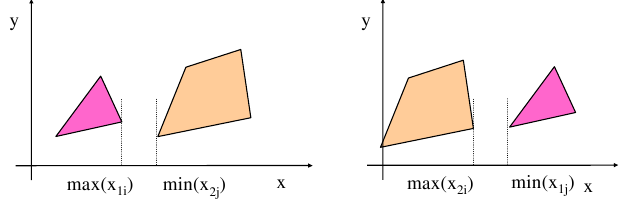
\includegraphics[height=2.5cm]{slike/04_minmax_1.png}
	\end{center}
\end{frame}

\begin{frame}{Min-maks contd.}
	\begin{center}
		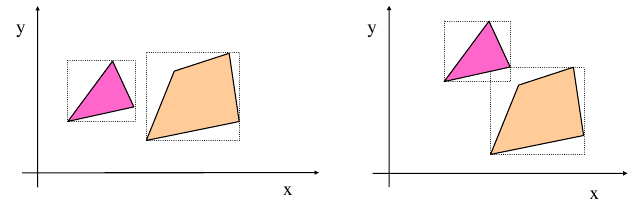
\includegraphics[height=2.5cm]{slike/04_minmax_2.png}
	\end{center}
	Potrebno naći da li se opisani pravokutnici(screen extent) prekrivaju 
	\begin{center}
		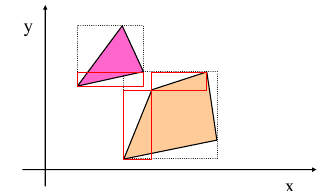
\includegraphics[height=2.5cm]{slike/04_minmax_3.png}
	\end{center}
	Algoritam se može primijeniti na bridove\\
	Ukoliko se prekrivaju, potrebne se daljnje provjere
\end{frame}

\begin{frame}{Min-maks contd.}
	\begin{block}{Proširenje na 3D}
		Provjerava se da li se kvadri (eng. bounding box), koji obuhvaćaju tijela
		ili dijelove tijela preklapaju. Postupak se obično koristi kod detekcije
		kolizije. Umjesto kvadara često se koriste kugle (sfere). 
	\end{block}
	\begin{block}{Primjer}
		Ukoliko je udaljenost pravca do središta kugle:\\
		\begin{itemize}
			\item veća od polumjera, pravac ne siječe kuglu.
			\item manja od polumjera, pravac siječe kuglu.
		\end{itemize}
	\end{block}
\end{frame}

%\begin{frame}{Min max provjera}
%	\begin{center}
%		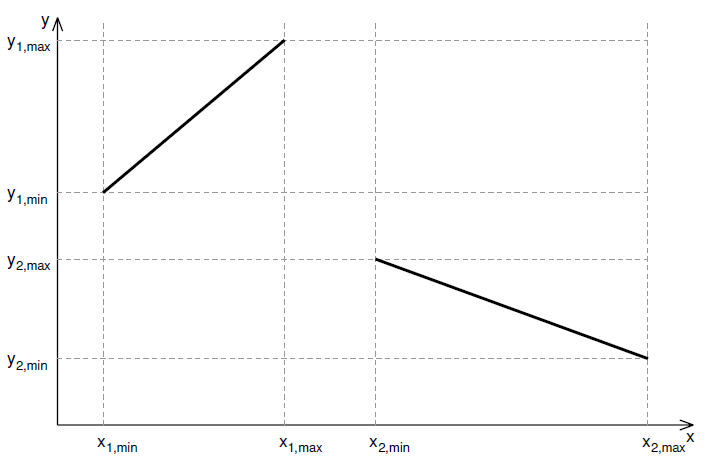
\includegraphics[height=2.5cm]{./slike/minmax01.png}
%		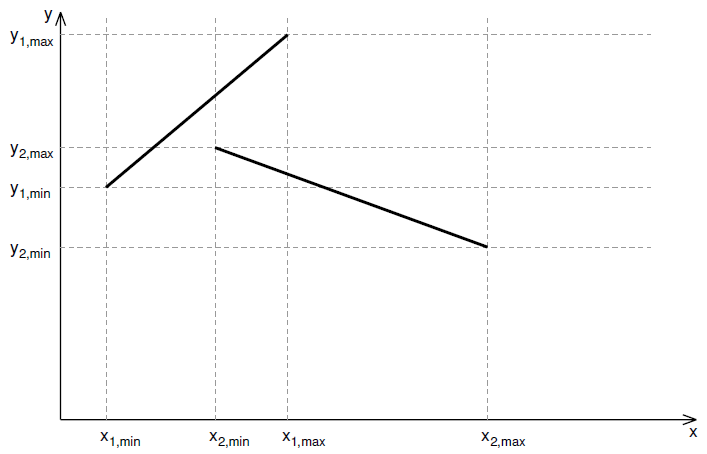
\includegraphics[height=2.5cm]{./slike/minmax02.png}
%	\end{center}
%\end{frame}
%\begin{frame}{Min max provjera}
%	\begin{center}
%		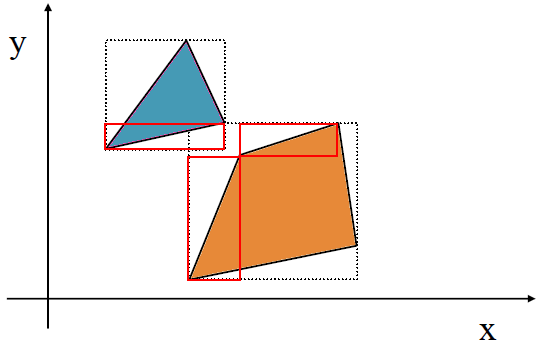
\includegraphics[height=2.5cm]{./slike/minmax03.png}
%	\end{center}
%\end{frame}
%\section{Watkinsov algoritam}

\section{Z spremnik}
\begin{frame}{Z spremnik}
	\begin{figure}
		\centering
		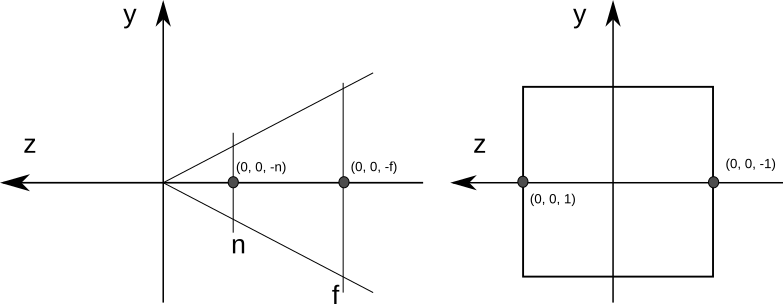
\includegraphics[width=0.7\textwidth]{slike/p04_07.png}
	\end{figure}
\end{frame}
\section{Warnockov postupak}

\begin{frame}{Warnock-ov postupak}
	Divide and conquer algoritam\\
	Analizira se sadržaj ispitnog prostora koji je u početku jednak zaslonu.\\
	Dosegnuta unaprijed zadana dubina rekurzije(prazno)\\
	(1)-(4) prozor je prazan ili je scena u prozoru jednostavna (\begin{tiny}Ne više od jednog poligona\end{tiny})\\
	(0) - scena u prozoru je složena, rekurzivno se dijeli dalje
	\begin{center}
		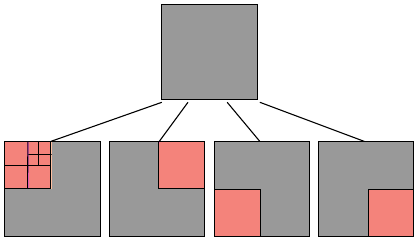
\includegraphics[height=4cm]{slike/05_warnock_1.png}
	\end{center}
\end{frame}

\begin{frame}{Podjela prostora}
	\begin{block}{Poligone se dijeli s obzirom na relaciju s prozorom}
		\begin{enumerate}
			\item poligon je izvan prozora (izbacuje se iz liste)
			\item Poligon siječe prozor ili je u prozoru
			\item Poligon prekriva prozor
			\item Više poligona prekriva ili siječe prozor
			\begin{itemize}
				\item daljnje ispitivanje - ako je poligon najbliži onda (4)
				\item inače (0)
			\end{itemize}
		\end{enumerate}
	\end{block}
	\begin{center}
		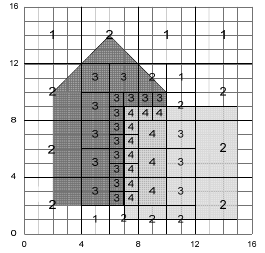
\includegraphics[height=3cm]{slike/05_warnock_1a.png}
	\end{center}
\end{frame}

\begin{frame}{Daljnje ispitivanje}
%	Ako je poligon koji prekriva prozor najbliži po udaljenosti od promatrača
	\begin{itemize}
		\item odredimo za svaki poligon ravninu u kojoj leži taj poligon i za tu ravninu odredimo z-koordinate u vrhovima promatranog prozora
		\begin{itemize}
			\item ako je poligon koji prekriva prozor najbliži promatraču tada je to slučaj (4)
			\item inače je scena u prozoru složena i dijelimo dalje, slučaj (0)
		\end{itemize}
	\end{itemize}
	\begin{center}
		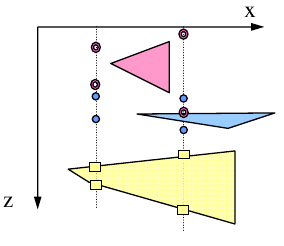
\includegraphics[height=3cm]{slike/05_warnock_2.png}
		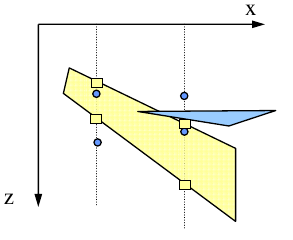
\includegraphics[height=3cm]{slike/05_warnock_3.png}
	\end{center}
\end{frame}

%\begin{frame}{Warnockov}
%	\begin{center}
%		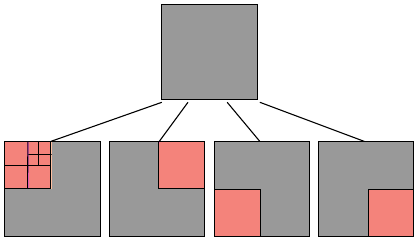
\includegraphics[height=2.5cm]{./slike/05_warnock_1.png}
%	\end{center}
%\end{frame}
%
%\begin{frame}{Warnockov}
%	\begin{center}
%		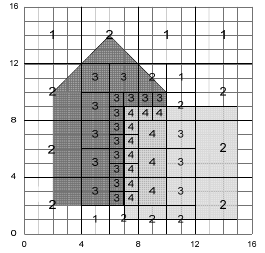
\includegraphics[height=2.5cm]{./slike/05_warnock_1a.png}
%	\end{center}
%\end{frame}
%
%
%\begin{frame}{Warnockov}
%	\begin{center}
%		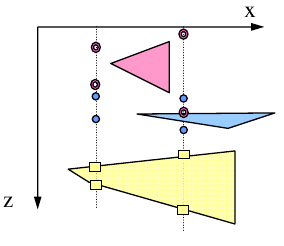
\includegraphics[height=2.5cm]{./slike/05_warnock_2.png}
%	\end{center}
%\end{frame}
%
%\begin{frame}{Warnockov}
%	\begin{center}
%		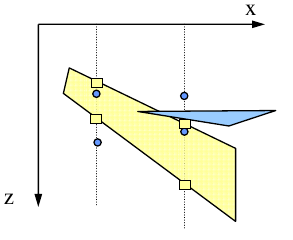
\includegraphics[height=2.5cm]{./slike/05_warnock_3.png}
%	\end{center}
%\end{frame}

\section{Četvero i oktalno stablo}
\begin{frame}{Slika s interneta}
	\begin{figure}
		\centering
		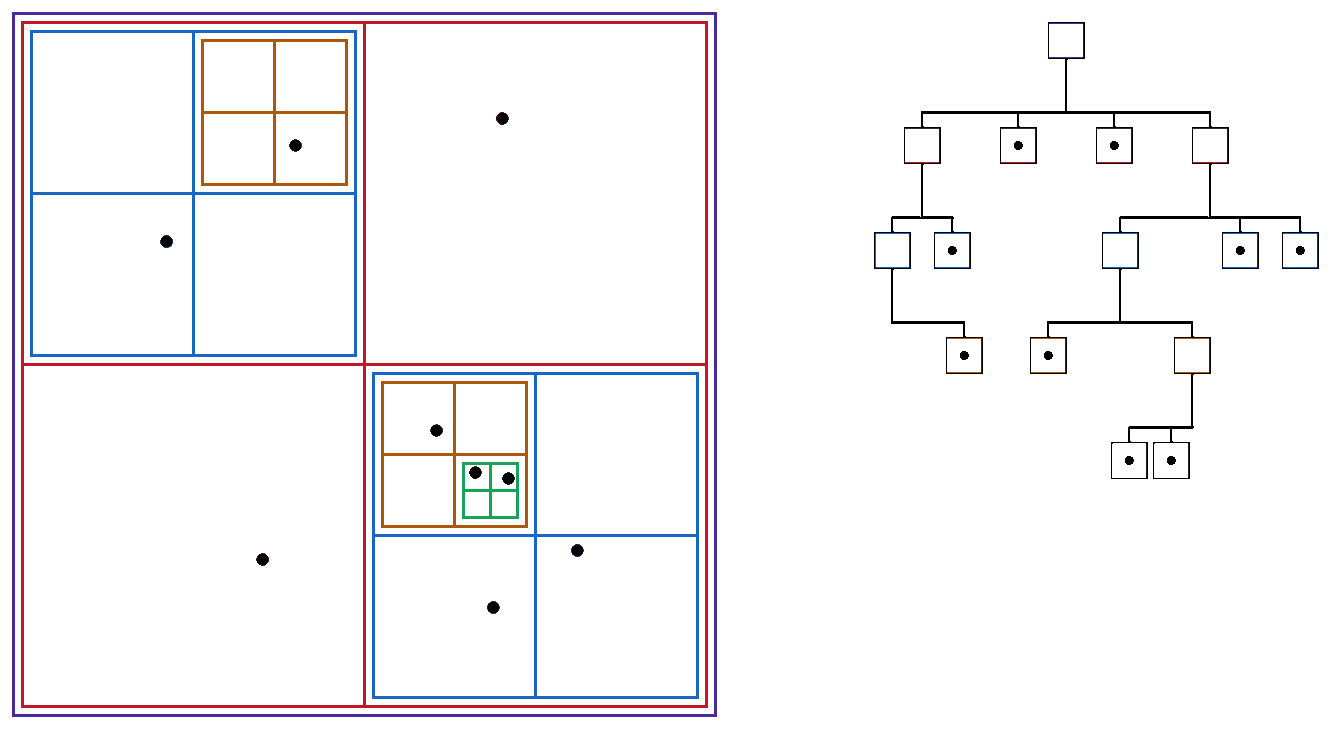
\includegraphics[width=0.7\linewidth]{./slike/quadtree.png}
	\end{figure}
\begin{itemize}
	\item Stablo, svaki čvor je završni ili ima 4 grane.
	\item Stablo se rekurzivno dijeli
	\item Uvjet zaustavljanja je unaprijed zadana dubina i/ili broj primitiva manji od unaprijed zadanog broja.
	\item Brza pretraga prostora
	\item k-d stablo
\end{itemize}
\end{frame}

\section{Cohen Sutherlandov algoritam}
\begin{frame}{Odsijecanje linije, 2D}
	\begin{columns}[t]
		\begin{column}{0.6\textwidth}
			\begin{itemize}
				\item Odsijecanje točaka
				\begin{itemize}
					\item Ako je $x_{min} < x < x_{max}$ i $y_{min} < y < y_{max}$, točka je unutar poligona
				\end{itemize}
				\item Endpoints:
				\begin{itemize}
					\item Ako su obje točke unutra, ?
					\item Jedna točka unutar, druga izvan, clip
					\item obje izvan - izvan ili clipped
				\end{itemize}
				\item Brute force clip: riječiti jednadžbe $y = mx+b$ za liniju i za četiri edge-a
				\begin{itemize}
					\item Neugodno za vertikalne linije, paralelne linije
				\end{itemize}
			\end{itemize}
		\end{column}
		\begin{column}{0.4\textwidth}
			\begin{center}
				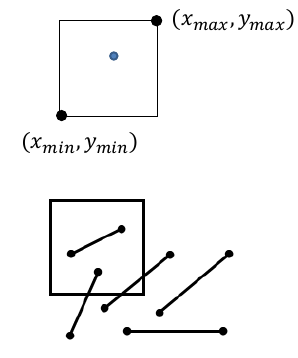
\includegraphics[width=5cm]{slike/line_clip_2d.png}
			\end{center}
		\end{column}
	\end{columns}
\end{frame}

\begin{frame}{Odsijecanje linije, 2D, parametarska formulacija}
	\begin{itemize}
		\item Jednadžba:
		\begin{itemize}
			\item $x = x_{0}+t(x_{1}-x_{0})$
			\item $y = y_{0}+t(y_{1}-y_{0})$
			\item $P(t) = P_{0}+t(P_{1}-P_{0})=(1-t)P_{0}+tP_{1}$
		\end{itemize}
		\item Linija je unutar pravokutnika ako su $t_{line}$ i $s_{edge}$ unutar $[0,1]$ na sjecištu
		između linije i edge-a:
		\begin{itemize}
			\item sporo, sporo, sjecište svih linija sa svima
		\end{itemize}
	\end{itemize}
	\begin{center}
		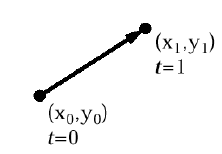
\includegraphics[width=3cm]{slike/parametric.png}
		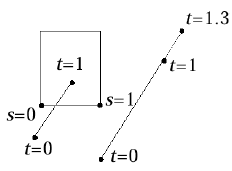
\includegraphics[width=3cm]{slike/parametric_2.png}
	\end{center}
\end{frame}
\begin{frame}{Odsijecanje linije, 2D, Cohen-Sutherland}
	\begin{itemize}
		\item Podijeliti ravninu na 9 područja:
		\item Izračunati \textsl{sign bit} četiri usporedbe između verteksa i edge-a.
		\begin{itemize}
			\item $x_{max}- x;  x-x_{min}; y_{max}-y;  y-y_{min};$
			\item Točka leži unutar samo aku su sva četiri \textsl{sign bits}=0
		\end{itemize}
		\item 4bit kod:
		\begin{itemize}
			\item Prvi bit: iznad gornjeg edge-a
			\item Drugi bit: ispod donjeg edge-a
			\item Treći bit: desno od desnog edge-a
			\item Četvrti bit: lijevo od lijevog edge-a
		\end{itemize}
		\item Izračunati kodove za oba verteksa svake linije ($OC_{0}$ i $OC_{1}$)
		\item Linije sa $OC_{0} = 0$(tj. $0000$) i $OC_{1}=0$?
		\item Linije koje leže potpuno izvan na način da vrijedi $OC_{0}\neq0$ i $OC_{1}\neq0$ (tj. dijele vanjski bit)?
	\end{itemize}
	\begin{center}
		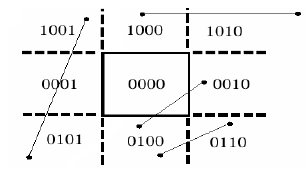
\includegraphics[width=3cm]{slike/clip_rect.png}
	\end{center}
\end{frame}

\begin{frame}{Odsijecanje linije, 2D, Cohen-Sutherland, contd.}
	\begin{itemize}
		\item Ako je nemoguće prihvatiti ili odbaciti liniju:
		\item Podijeliti liniju da dva segmenta; onda acc ili rej jedan ili oba segmenta:
		\begin{itemize}
			\item Upotrijebiti clip edge za odsijecanje linije
			\item upotrijebiti kodove za odabir edgev-a koji su prijeđeni
			\item odabrati poredak za provjeru edgev-a: top-bottom-right-left
			\item izračunati točku sjecišta - fiksiramo x ili y
			\item iteriramo sa novom kraćom linijom, mogu se pojaviti ekstra clips
		\end{itemize}
	\end{itemize}
	\begin{center}
		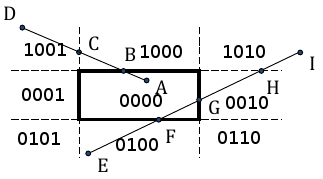
\includegraphics[width=5cm]{slike/clip_rect_2.png}
	\end{center}
\end{frame}

\section{Cyrus Beckov algoritam}
\begin{frame}{Cyrus Beck}
	\begin{block}{}
		\begin{itemize}
			\item Unaprijeđeni Cohen Sutherlandov algoritam
			\item Probodište pravca sa proizvoljnim konveksnim poliedrom.
		\end{itemize}
	\end{block}
Ako je zadano:
\begin{itemize}
	\item $P(t) = t(P_1-P_0) + P_0$
	\item točka na poligonu $P_p$
	\item normala poligona $\vec{n}$
\end{itemize}
Probodište:
\begin{align*}
\vec{n}\left( P(t) - P_p\right)=0
\end{align*}
Uvrsti li se u jednadžbu pravca:
\begin{align*}
t = \frac{\vec{n}\left(P_0-P_p\right)}{-\vec{n}D}
\end{align*}
Ovdje je $D = P_1-P_0$
\end{frame}
\begin{frame}{Cyrus Beck}
	\begin{figure}
		\centering
		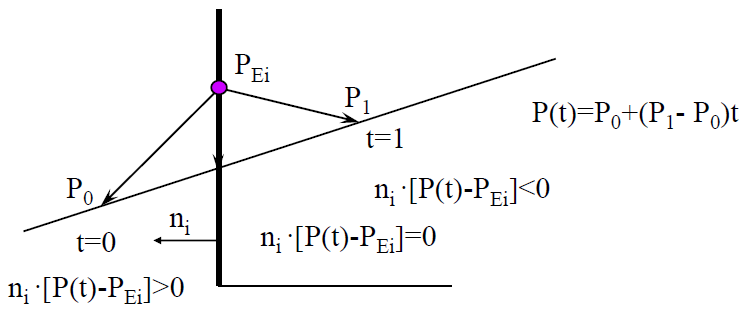
\includegraphics[width=0.7\linewidth]{slike/cyrus_beck01.png}
	\end{figure}
\end{frame}
\begin{frame}{Cyrus Beck}
	\begin{figure}
		\centering
		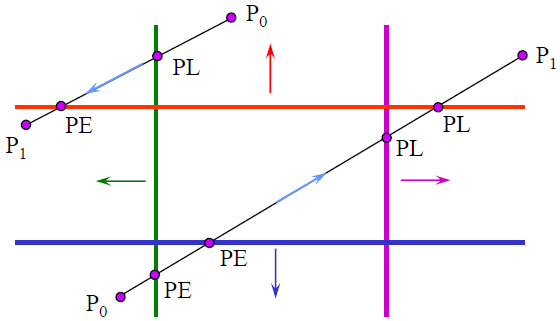
\includegraphics[width=0.7\linewidth]{slike/cyrus_beck02.png}
	\end{figure}
	\begin{itemize}
		\item $PE=0$ i $PL=1$
		\item $\vec{n}D < 0$, sjecište je $PE$, inače $PL$
		\item Odabrati najveći $PE$ i najmanji $PL$
		\item Ako je $PE<PL$, onda imamo traženo odsijecanja  
	\end{itemize}
\end{frame}
\section{Binarna podjela prostora}

\begin{frame}{BSP}
	\begin{itemize}
		\item Binarno stablo
		\item Sortiramo poligone, koji je ispred a koji iza
		\item Svaki čvor sadrži normalu i poligon
		\item Ako se ne može odrediti je li poligon ispred ili iza, onda se radi split
		\item Problem ako je stablo skoro sortirano, ili su sortirane grupe
		\item Poligoni se dijele na vrlo male podpoligone
		\item Poligoni mogu biti geometrijski daleko i uzrokovati dijeljenje
		\item Nije potrebno generirati stablo svakim pomakom kamere
	\end{itemize}
	\begin{figure}
		\centering
		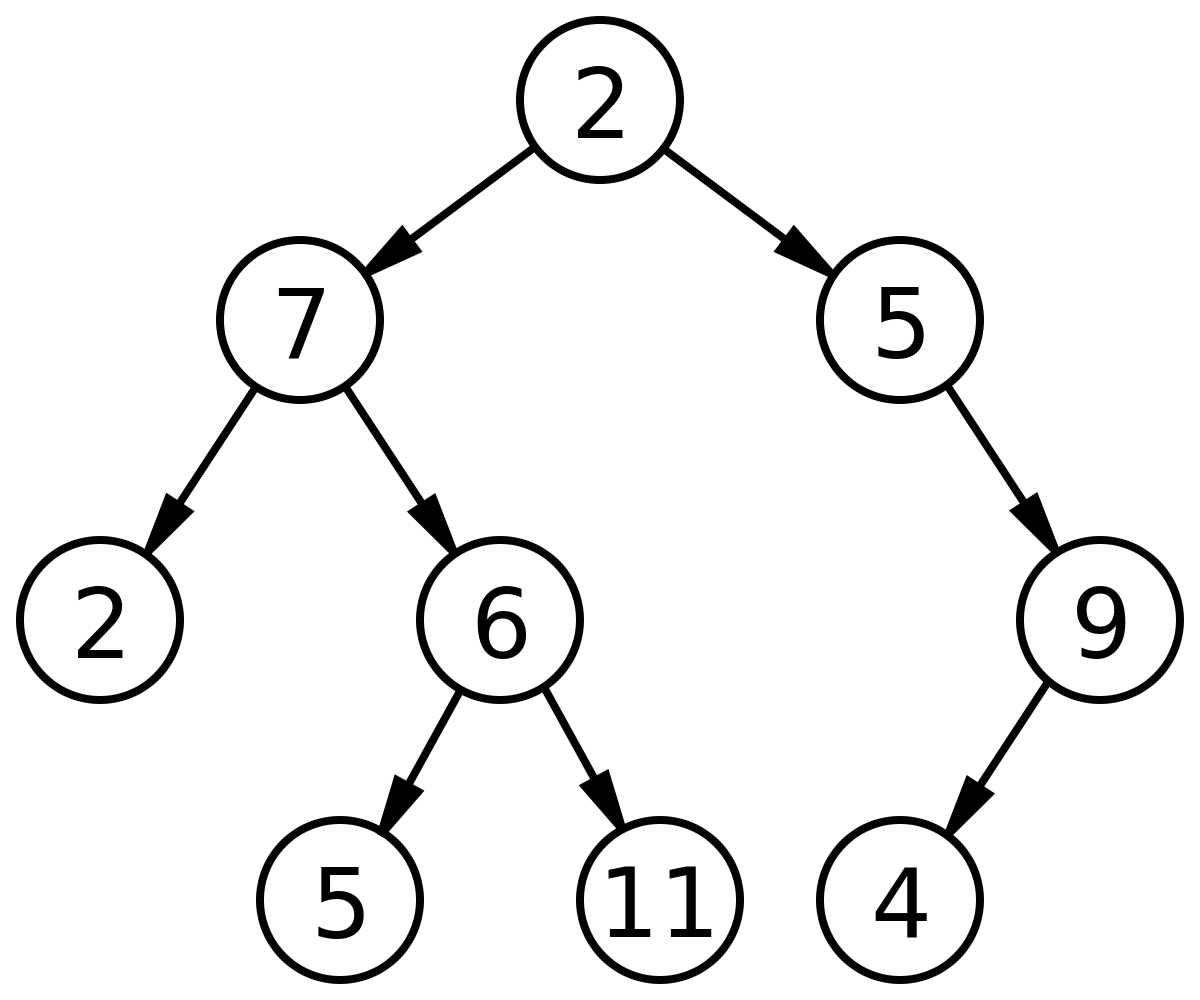
\includegraphics[width=4cm]{slike/binary_tree.png}
	\end{figure}
\end{frame}
\plain{Pitanja?}
\end{document}